\section{Object Space Volume Rendering}
In object space rendering methods the main loop is not over the pixels but over the objects in $3$-space. In case of direct volume rendering "objects" can mean:
\begin{itemize}
    \item Layers of voxels: Use \emph{Image compositing} methods:
        \begin{itemize}
            \item 2D texture based
            \item 3D texture based
        \end{itemize}
    \item Voxels: Use \emph{splatting} methods.
    \item Cells: Use \emph{cell projection} methods.
\end{itemize}

\subsection{Texture-based volume rendering}
\subsubsection{Volume rendering with 2D texturemapping}
\begin{itemize}
    \item Use planes parallel to the \emph{base plane}. The base plane is the front face of the volume which is "most orthogonal" to the view ray.
    \item Draw the texture rectangles using a bilinear interpolation filter.
    \item Render back-to-front using $\alpha$-blending for the $\alpha$-composition.
\end{itemize}
\begin{figure}[H]
    \centering
    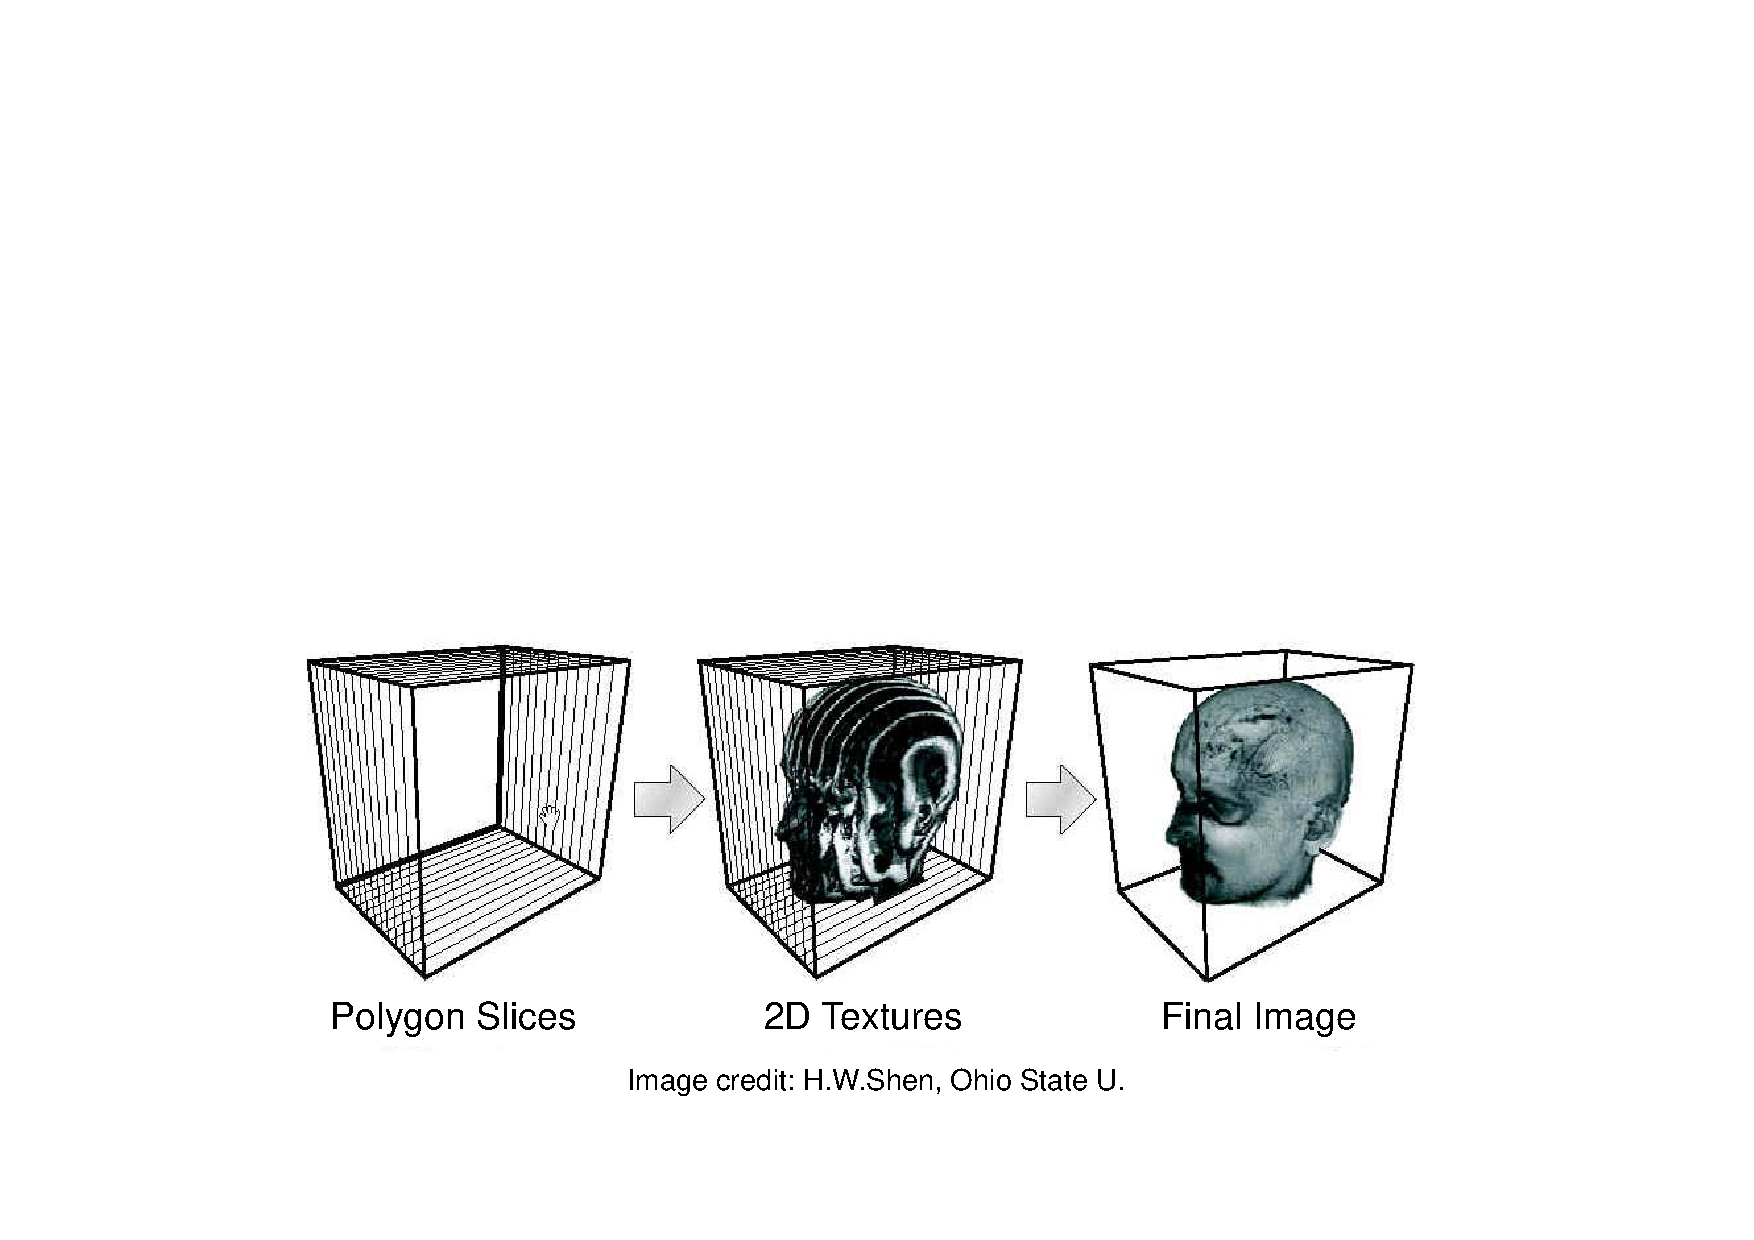
\includegraphics[width=0.8\textwidth]{img/04_texture_based_volume_rendering}
\end{figure}

\subsubsection{Volume rendering with 3D texture mapping}
Cabral 1994.
\begin{itemize}
    \item Use the voxel data as the 3D texture.
    \item Render an arbitrary number of slices (eg. 100 or 1000) parallel to the image plane (3- to 6- sided polygons).
    \item Back-to-front compositing as in the 2D texture method.
\end{itemize}
This method is limited by the size of the texture memory. 
\begin{figure}[H]
    \centering
    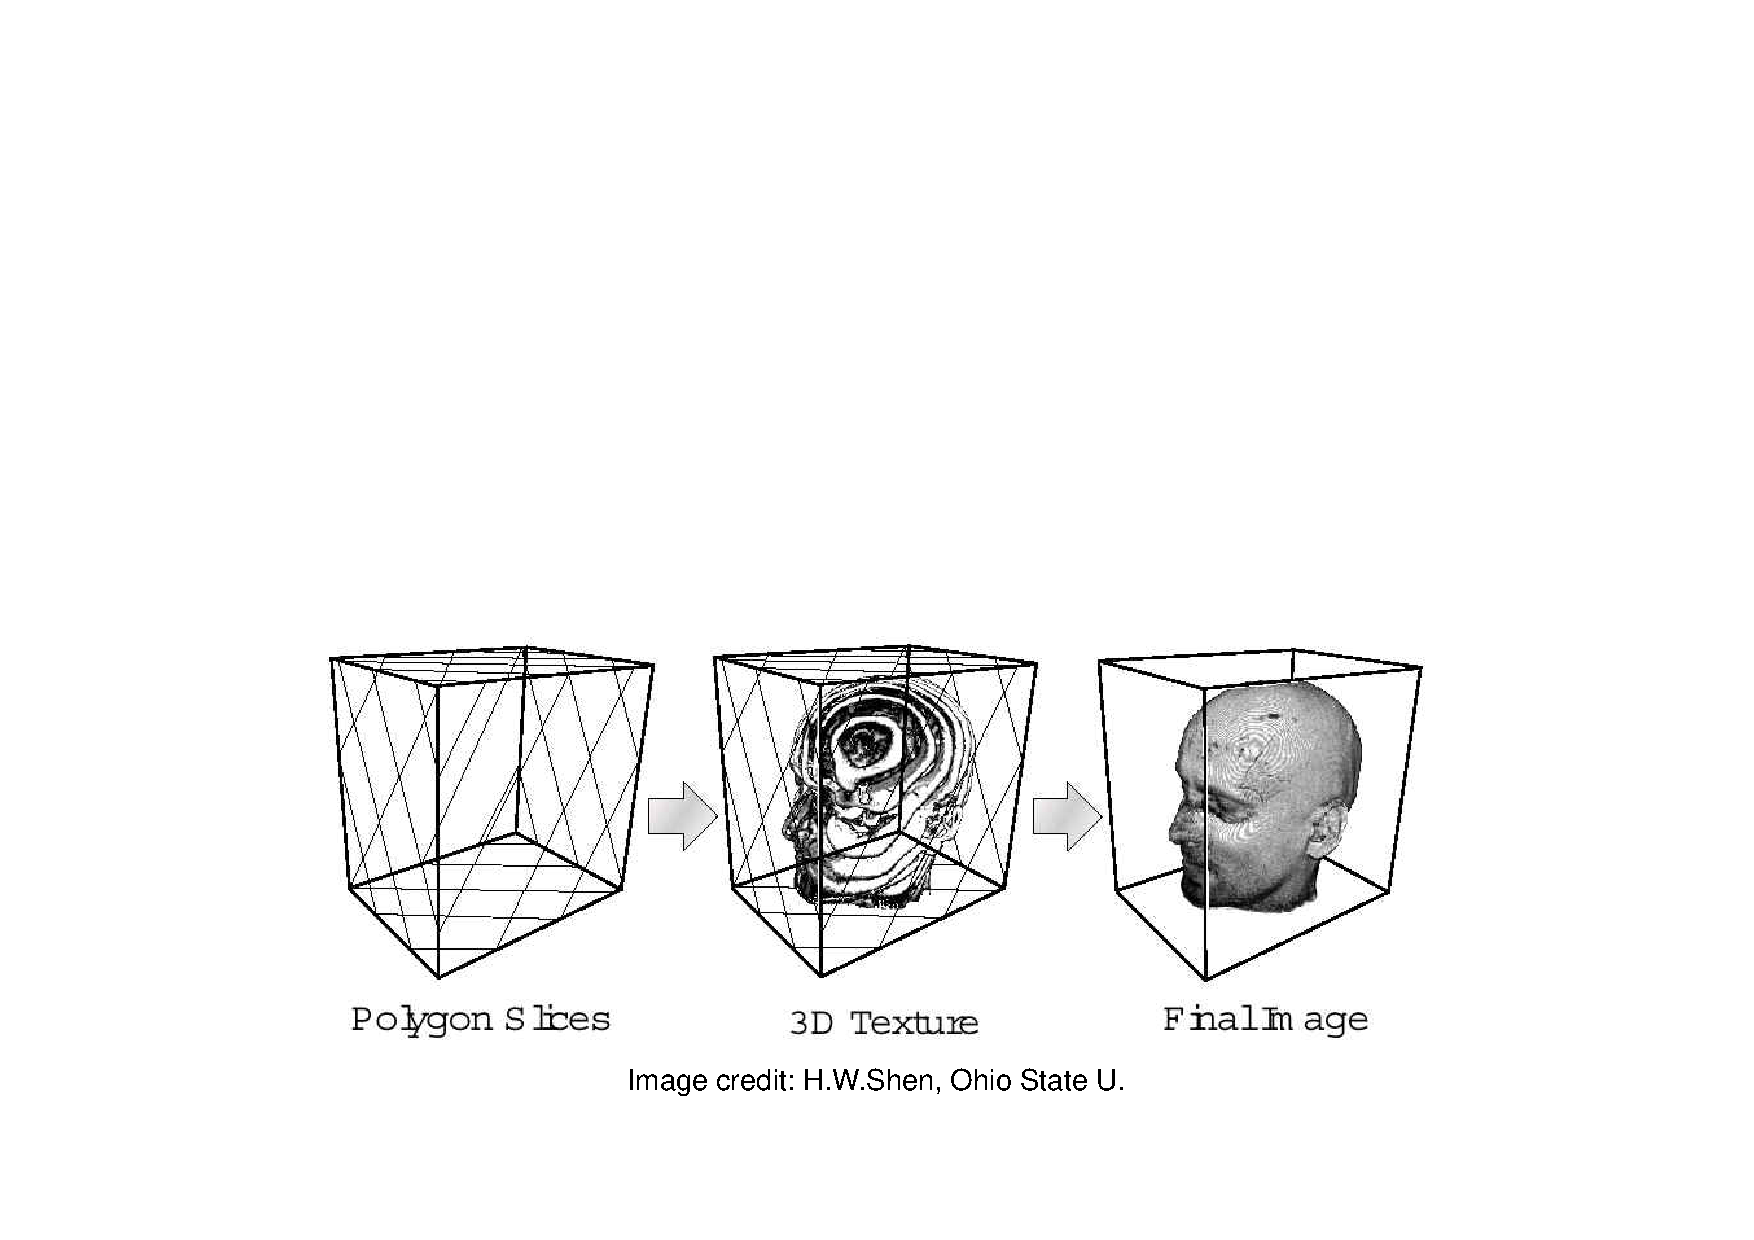
\includegraphics[width=0.8\textwidth]{img/04_3dtexture_based_volume_rendering}
\end{figure}

\subsection{Shear-Warp Factorisation}
In general the image plane is not parallel to a volume face. The \emph{shear-warp} method allows to render an intermediate image in the base plane:
\begin{enumerate}
    \item Transform the \emph{sheared object space} by translating (and possibly scaling) the voxel layers.
    \item \emph{Render} the intermediate image in the base plane.
    \item \emph{Warp} the intermediate image.
\end{enumerate}
\begin{figure}[H]
    \centering
    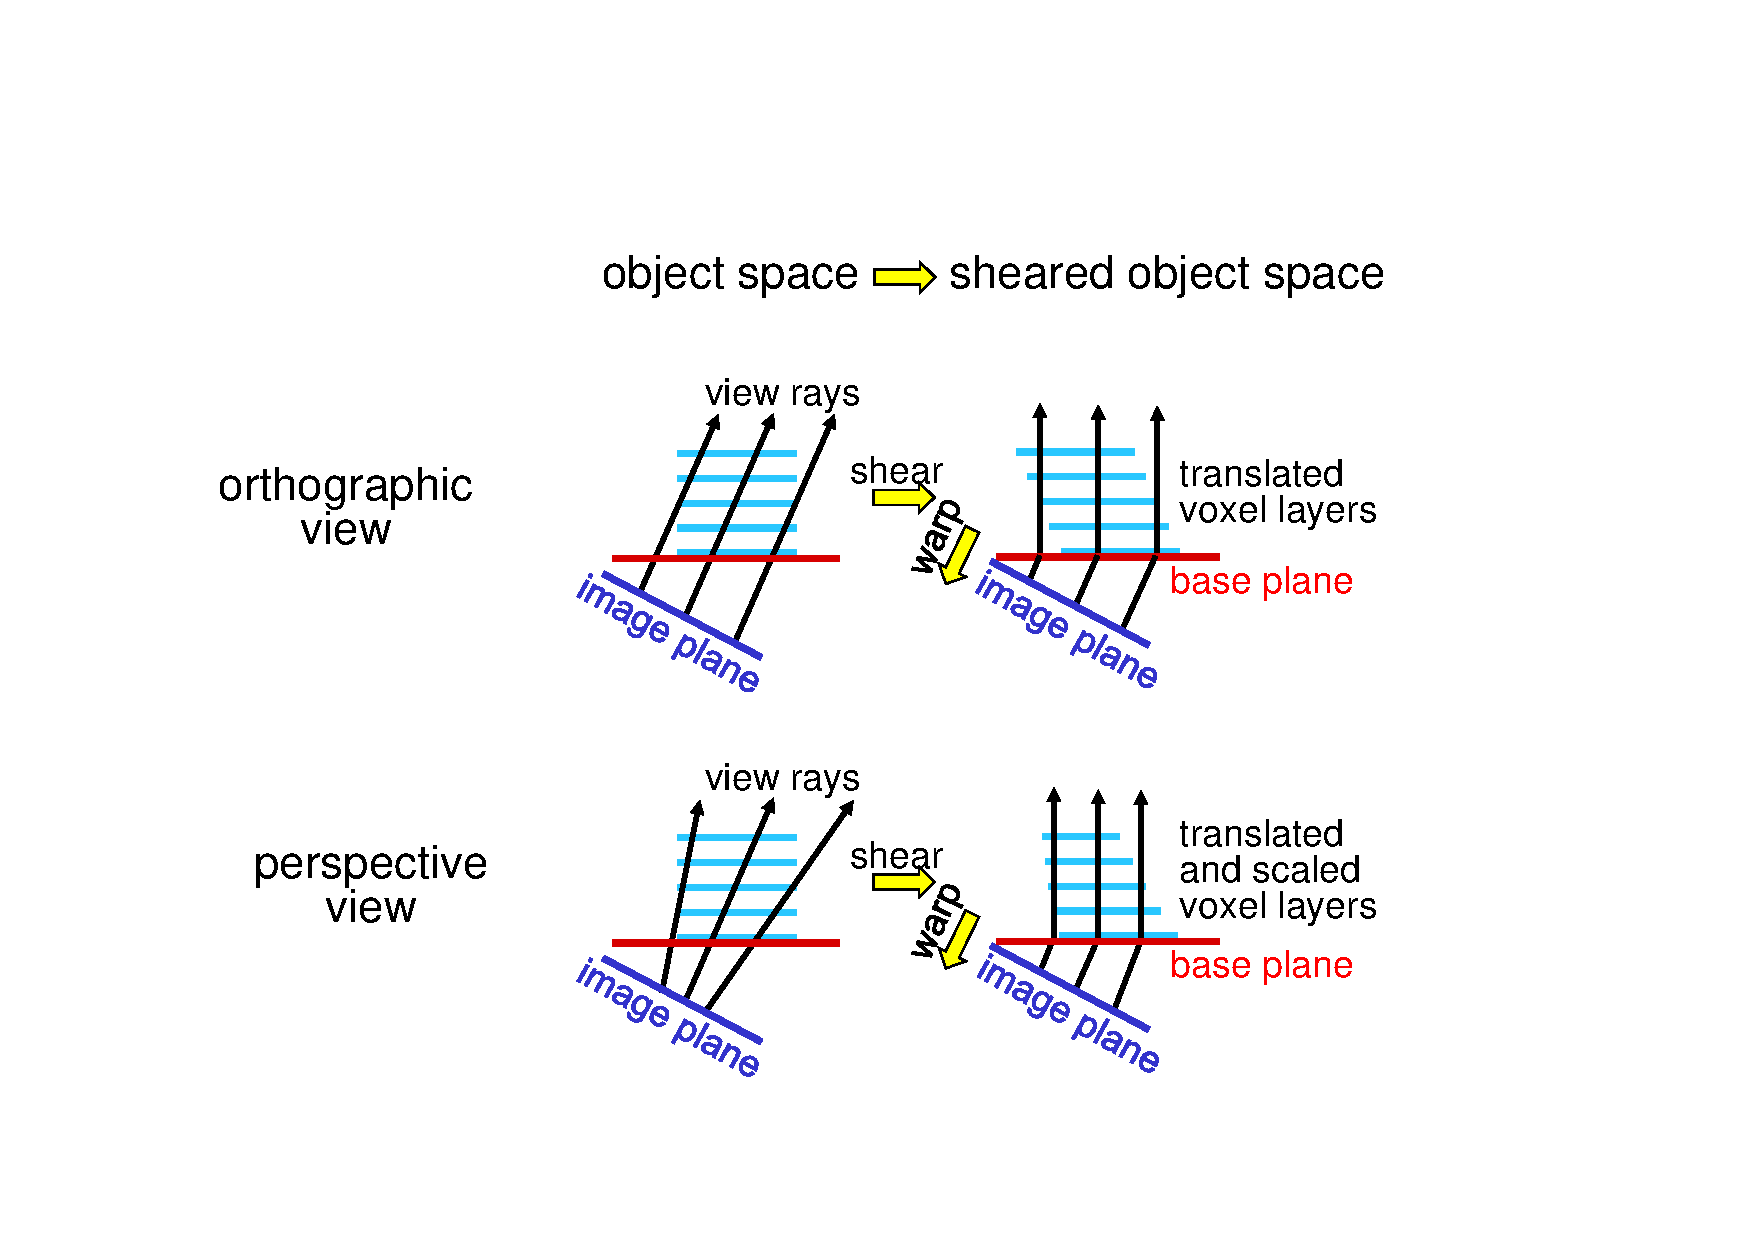
\includegraphics[width=0.8\textwidth]{img/04_shear_warp_overview}
\end{figure}

The \emph{view transformation} is an affine transformation consisting of a rotation and a translation. Ignoring the translation, the $3\times 3$ matrix can be factorised:
\begin{align*}
    M_\text{view} = W\cdot S \cdot P
\end{align*}
where
\begin{itemize}
    \item $P$ is a permutation matrix mapping the base plane to the $xy$ plane.
    \item $S$ is the shear matrix. The \emph{shear} is of the form
        \begin{align*}
            S
            \begin{pmatrix}
                x\\
                y\\
                z
            \end{pmatrix} =
            \begin{pmatrix}
                x\\
                y\\
                z
            \end{pmatrix} + z
            \begin{pmatrix}
                s_x\\
                s_y\\
                0
            \end{pmatrix}.
        \end{align*}
        With $S$ being:
        \begin{align*}
            S =
            \begin{pmatrix}
                1 & 0 & s_x\\
                0 & 1 & s_y\\
                0& 0& 1
            \end{pmatrix}
        \end{align*}
        where $s_x$ and $s_y$ have to be solved for from $M_\text{view}$.
    \item $W$ is the warp matrix. The \emph{warp} is a $3\times 3$ matrix and effectively an affine transformation of the $xy$-plane. The third row of $W$ is irrelevant while two zeros in the third column are required to make the warp independent of $z$.
    \begin{align*}
        W = 
            \begin{pmatrix}
                w_{00} & w_{01} & 0\\
                w_{10} & w_{11} & 0\\
                w_{20} & w_{21} & w_{22}
            \end{pmatrix}
    \end{align*}
\end{itemize}

Assuming for simplicity that $P$ is the identity, we get:
\begin{align*}
    M_\text{view} = \begin{pmatrix}
                         v_{00} & v_{01} & v_{02}\\
                         v_{10} & v_{11} & v_{12}\\
                         v_{20} & v_{21} & v_{22}
                    \end{pmatrix} = W\cdot S = 
            \begin{pmatrix}
                w_{00} & w_{01} & s_x w_{00} + s_y w_{01}\\
                w_{10} & w_{11} & s_x w_{10} + s_y w_{11}\\ 
                w_{20} & w_{21} & s_x w_{20} + s_y w_{21} + w_{22}
            \end{pmatrix}.
\end{align*}
It follows for the warp coefficients $w_{ij} = v_{ij}$ $(j\neq 2)$ and for the shear coefficients:
\begin{align*}
    \begin{pmatrix}
        s_x\\
        s_y 
    \end{pmatrix} =
    \begin{pmatrix}
        v_{00} & v_{01}\\
        v_{10} & v_{11} 
    \end{pmatrix}^{-1}
    \begin{pmatrix}
     v_{02}\\ v_{12}
    \end{pmatrix}
\end{align*}
and for $w_{22}$ (not needed):
\begin{align*}
    w_{22} = -s_x v_{20} -s_yv_{21} + v_{22}.
\end{align*}

If $P$ is not the identity, permuted versions of $S$ and $W$ can be used.

\subsection{Perspective shear warp}
The same factorisation as before can be used. But now \emph{homogeneous coordinates} are used:
\begin{align*}
    M_\text{view} = W\cdot S\cdot P.
\end{align*}
The \emph{shear and scaling} matrix $S$ gets the form
\begin{align*}
  S = 
    \begin{pmatrix}
     1&0&s_x&0\\
     0&1&s_y&0\\
     0&0&1&0\\
     0&0&s_w&1\\
    \end{pmatrix}.
\end{align*}
It does
\begin{itemize}
\item a translation of $x$ by $s_x z$ and of $y$ by $s_y z$ followed by
\item a scaling with ${1\over 1+s_w z}$.
\end{itemize}

The \emph{warp} matrix now is
    \begin{align*}
        W = 
            \begin{pmatrix}
                w_{00} & w_{01} & 0 & w_{03}\\
                w_{10} & w_{11} & 0 & w_{13}\\
                w_{20} & w_{21} & w_{22} & w_{23}\\
                w_{30} & w_{31} & 0 & w_{33}
            \end{pmatrix}.
    \end{align*}
Assuming again that $P$ is the identity we get:
\begin{align*}
    M_\text{view} = \begin{pmatrix}
                         v_{00} & v_{01} & v_{02} & v_{03}\\
                         v_{10} & v_{11} & v_{12} & v_{13}\\
                         v_{20} & v_{21} & v_{22} & v_{23}\\
                         v_{30} & v_{31} & v_{32} & v_{33}\\
                    \end{pmatrix} = W\cdot S = 
            \begin{pmatrix}
                w_{00} & w_{01} & s_x w_{00} + s_y w_{01} + s_w w_{03} & w_{03}\\
                w_{10} & w_{11} & s_x w_{10} + s_y w_{11} + s_w w_{13} & w_{13}\\ 
                w_{20} & w_{21} & s_x w_{20} + s_y w_{21} + w_{22} + + s_w w_{23} & w_{23}\\
                w_{30} & w_{31} & s_x w_{30} + s_y w_{31} + s_w w_{33} & w_{33}\\ 
            \end{pmatrix}.
\end{align*}
It follows that for the warp conditions $w_{ij} = v_{ij}$ with $(j\neq 2)$ holds.
For the shear coefficients:
\begin{align*}
    \begin{pmatrix}
        s_x\\
        s_y\\
        s_w
    \end{pmatrix} =
    \begin{pmatrix}
        v_{00} & v_{01} & v_{03}\\
        v_{10} & v_{11} & v_{13}\\
        v_{30} & v_{31} & v_{33}
    \end{pmatrix}^{-1}
    \begin{pmatrix}
     v_{02}\\ v_{12}\\ v_{32}
    \end{pmatrix}
\end{align*}
and for $w_{22}$ (not needed):
\begin{align*}
    w_{22} = -s_x v_{20} -s_yv_{21}-s_w v_{23} + v_{22}.
\end{align*}

For the shear-warp volume rendering algorithm now works as follows:
\begin{enumerate}
    \item For each voxel layer (parallel to base plane):
        \begin{itemize}
            \item Shear and scale the layer image by multiplying with $S$.
            \item Apply the transfer functions.
        \end{itemize}
    \item Generate intermediate image with $\alpha$ compositing.
    \item Warp the image by multiplying with $W$.
\end{enumerate}

An advantage of this algorithm is that an aliasing filter can be used to prevent undersampling when scaling the image.

\subsection{Object Space versus Image Space}
Comparison of the object space methods introduced and image space methods such as \emph{raycasting}.

Formally both methods are equivalent only the nesting order of the loops is different. Practical differences:
\begin{itemize}
    \item Image space methods with FTB compositing allow early termination.
    \item Object space methods using a framebuffer for intermediate results suffer from quantisation artefacts.
    \item Object space methods can exploit texture mapping hardware and MIPmap textures for antialiasing.
    \item Image space methods would need supersampling in $x$ and $y$ to get antialiasing.
\end{itemize}

\paragraph{Post-classification}
The post-classification can be done directly in the graphics hardware. Using (OpenGL) \emph{depndent texture} (two texture mapping stages):
\begin{figure}[H]
    \centering
    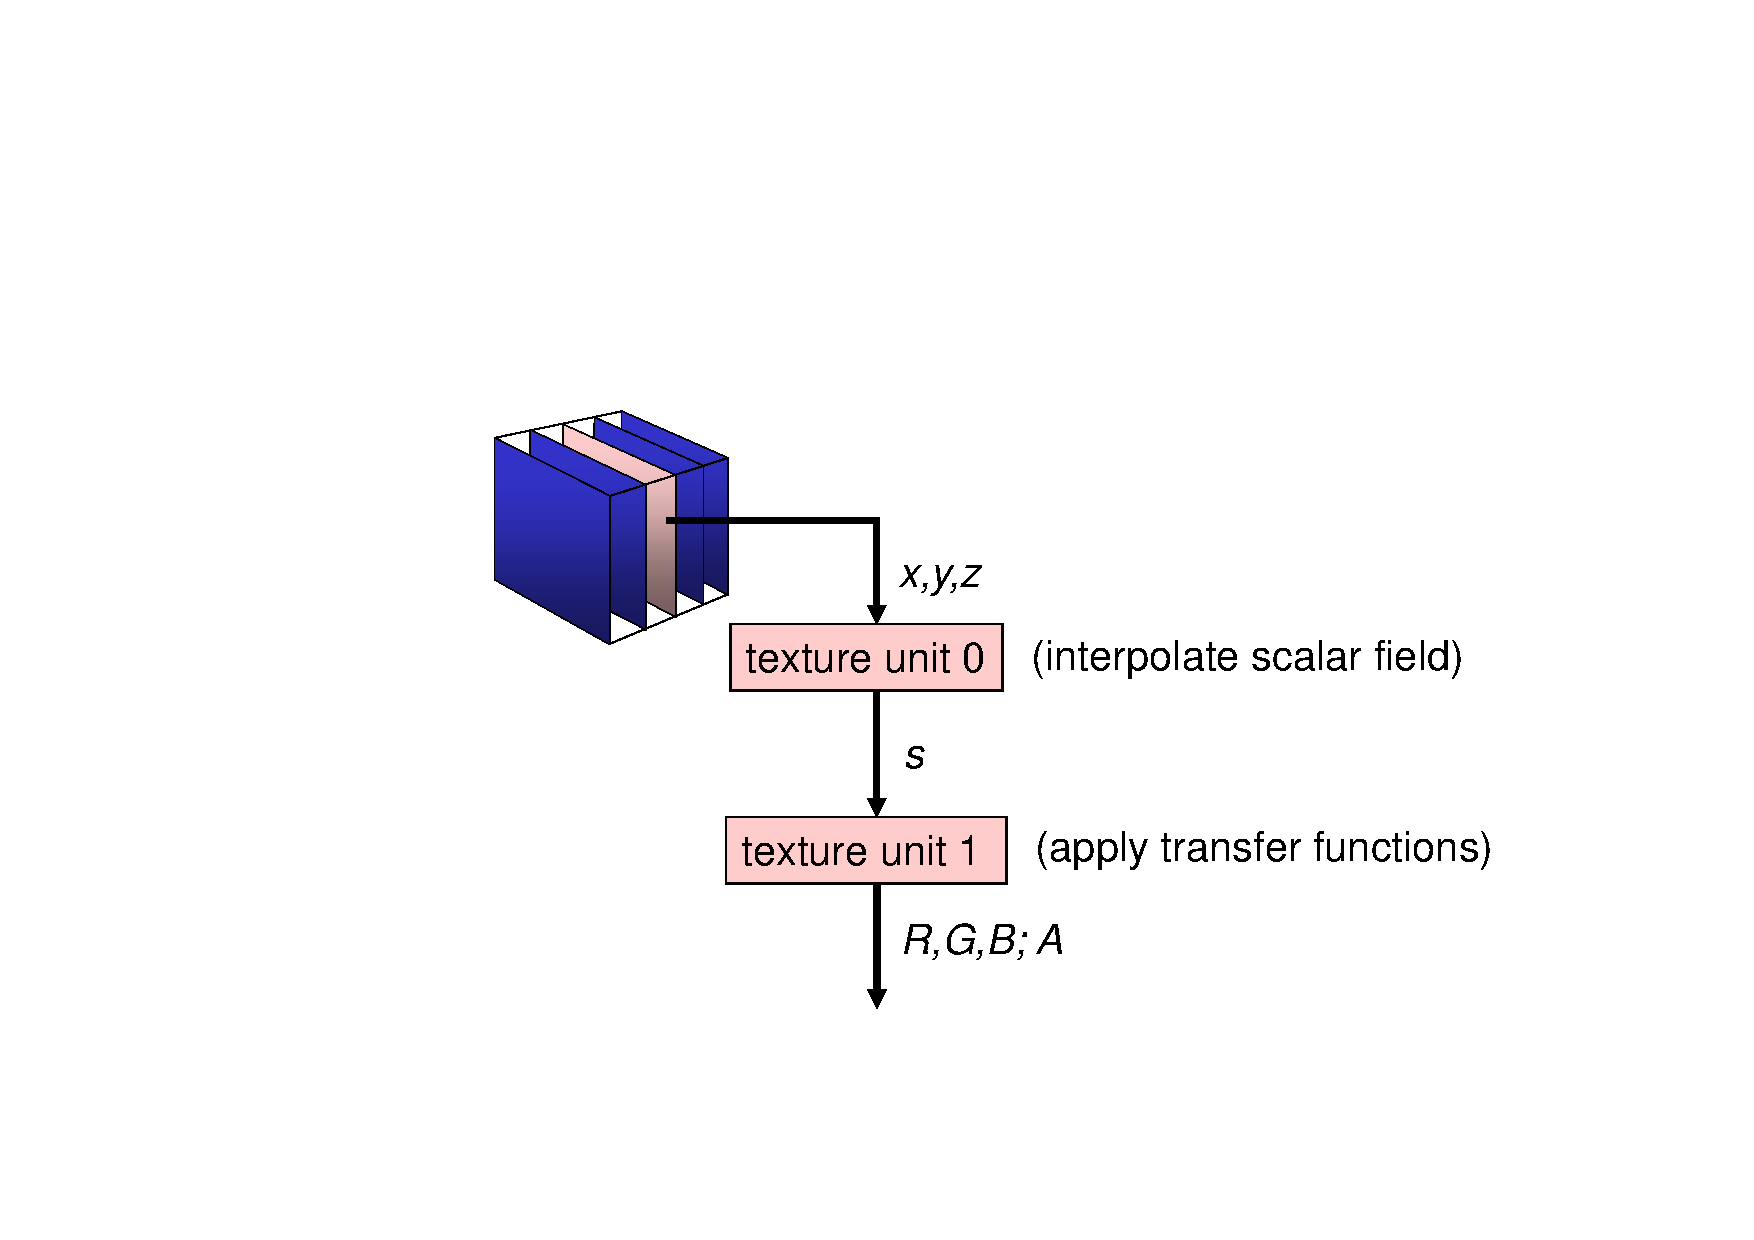
\includegraphics[width=0.6\textwidth]{img/04_object_space_dependent_texture}
\end{figure}

\paragraph{Pre-integration}
It's also possible to pre-integrate in object space:
\begin{itemize}
\item Use \emph{slabs} (space between two slices) and
\item Dependent textures:
    \begin{itemize}
        \item $1^{st}$ stage: Interpolate scalar filed in front and back slice.
        \item $2^{nd}$ stage: Look up integrated transfer function.
    \end{itemize}
\end{itemize}
\begin{figure}[H]
    \centering
    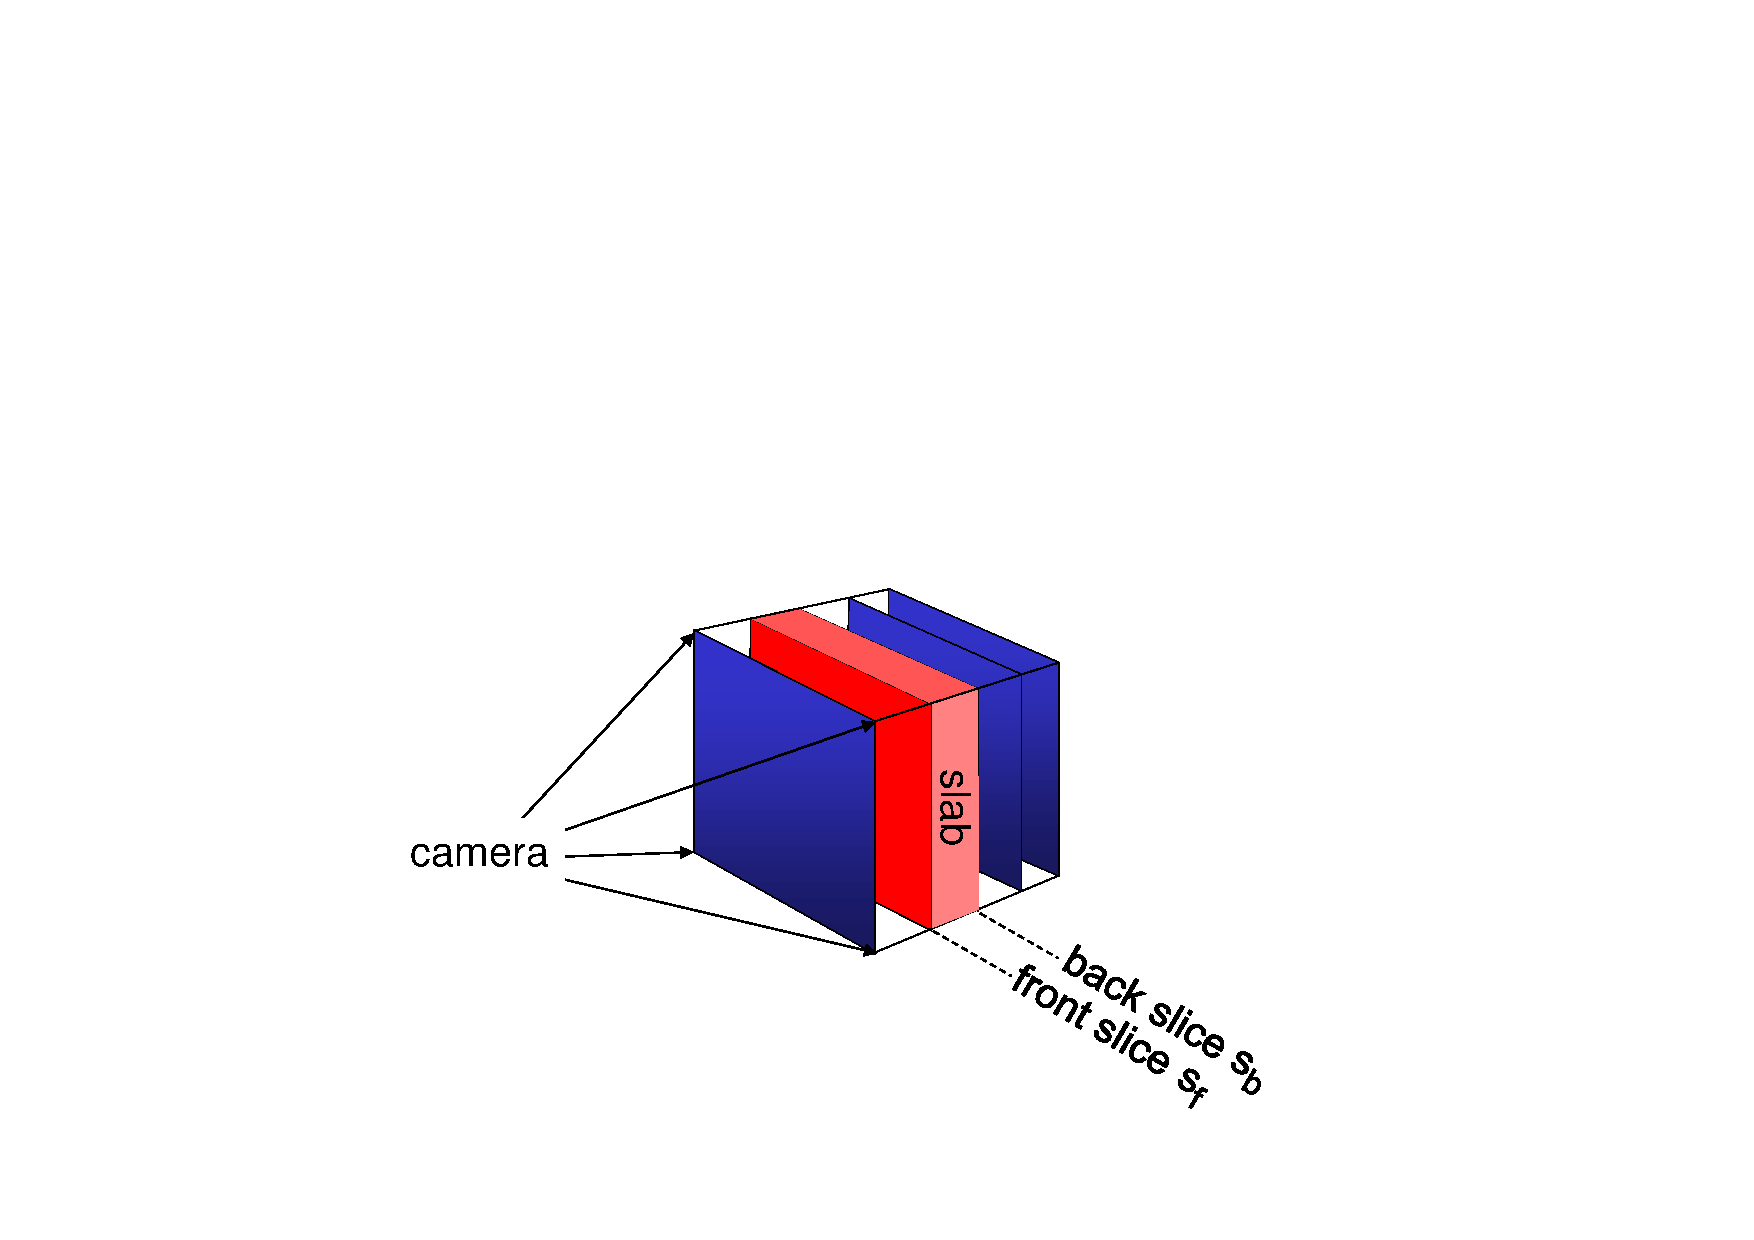
\includegraphics[width=0.6\textwidth]{img/04_object_space_preintegration}
\end{figure}

\subsection{Splatting}

\begin{description}
    \item[Raycasting] "What does \textbf{each} voxel contribute to a given pixel?"
    \item[Splatting] "What does \textbf{a given} voxel contribute to each pixel?"
\end{description}

Algorithm:
\begin{itemize}
    \item Pre-processing:
        \begin{itemize}
            \item For each voxel $x_i$ render (raycast) a field $s(x_i) = \delta_{ij}$.
            \item Store the resulting \emph{footprint} images.
        \end{itemize}
    \item Main loop:
        \begin{itemize}
            \item For each voxel $x_i$ adjust the footprint image to effective TF value.
            \item Do $\alpha$-compositing of all footprint images.
        \end{itemize}
\end{itemize}

Advantages of splatting:
\begin{itemize}
    \item Applicable to structured and unstructured grids.
    \item Other reconstruction filters than trilinear interpolation are possible (for example a sinc filter).
\end{itemize}

\paragraph{Original algorithm} Westover 1990: Orthographic view and uniform grids. All footprints are translations of a template.
\paragraph{Sheet buffer method} Westover 1991:
\begin{itemize}
    \item Blend all footprint images of a voxel layer ("sheet buffer")
    \item Do $\alpha$-compositing of sheet buffers.
\end{itemize}
\paragraph{Elliptical weighted average splatting} (EWA), Zwicker et al. 2001:
\begin{itemize}
    \item Ellipsoidal Gaussians are used as footprints
    \item Perspective view, low-pass filter for antialiasing.
\end{itemize}

\subsection{Cell Projection}
\emph{Projected tetrahedra} (PT) is an object space method for tetrahedral grids [Shirley, Tuchman 1990]. Each (tetrahedral) cell is decomposed into $3$ or $4$ tetrahedra along those edges which are not part of the silhouette.
\begin{figure}[H]
    \centering
    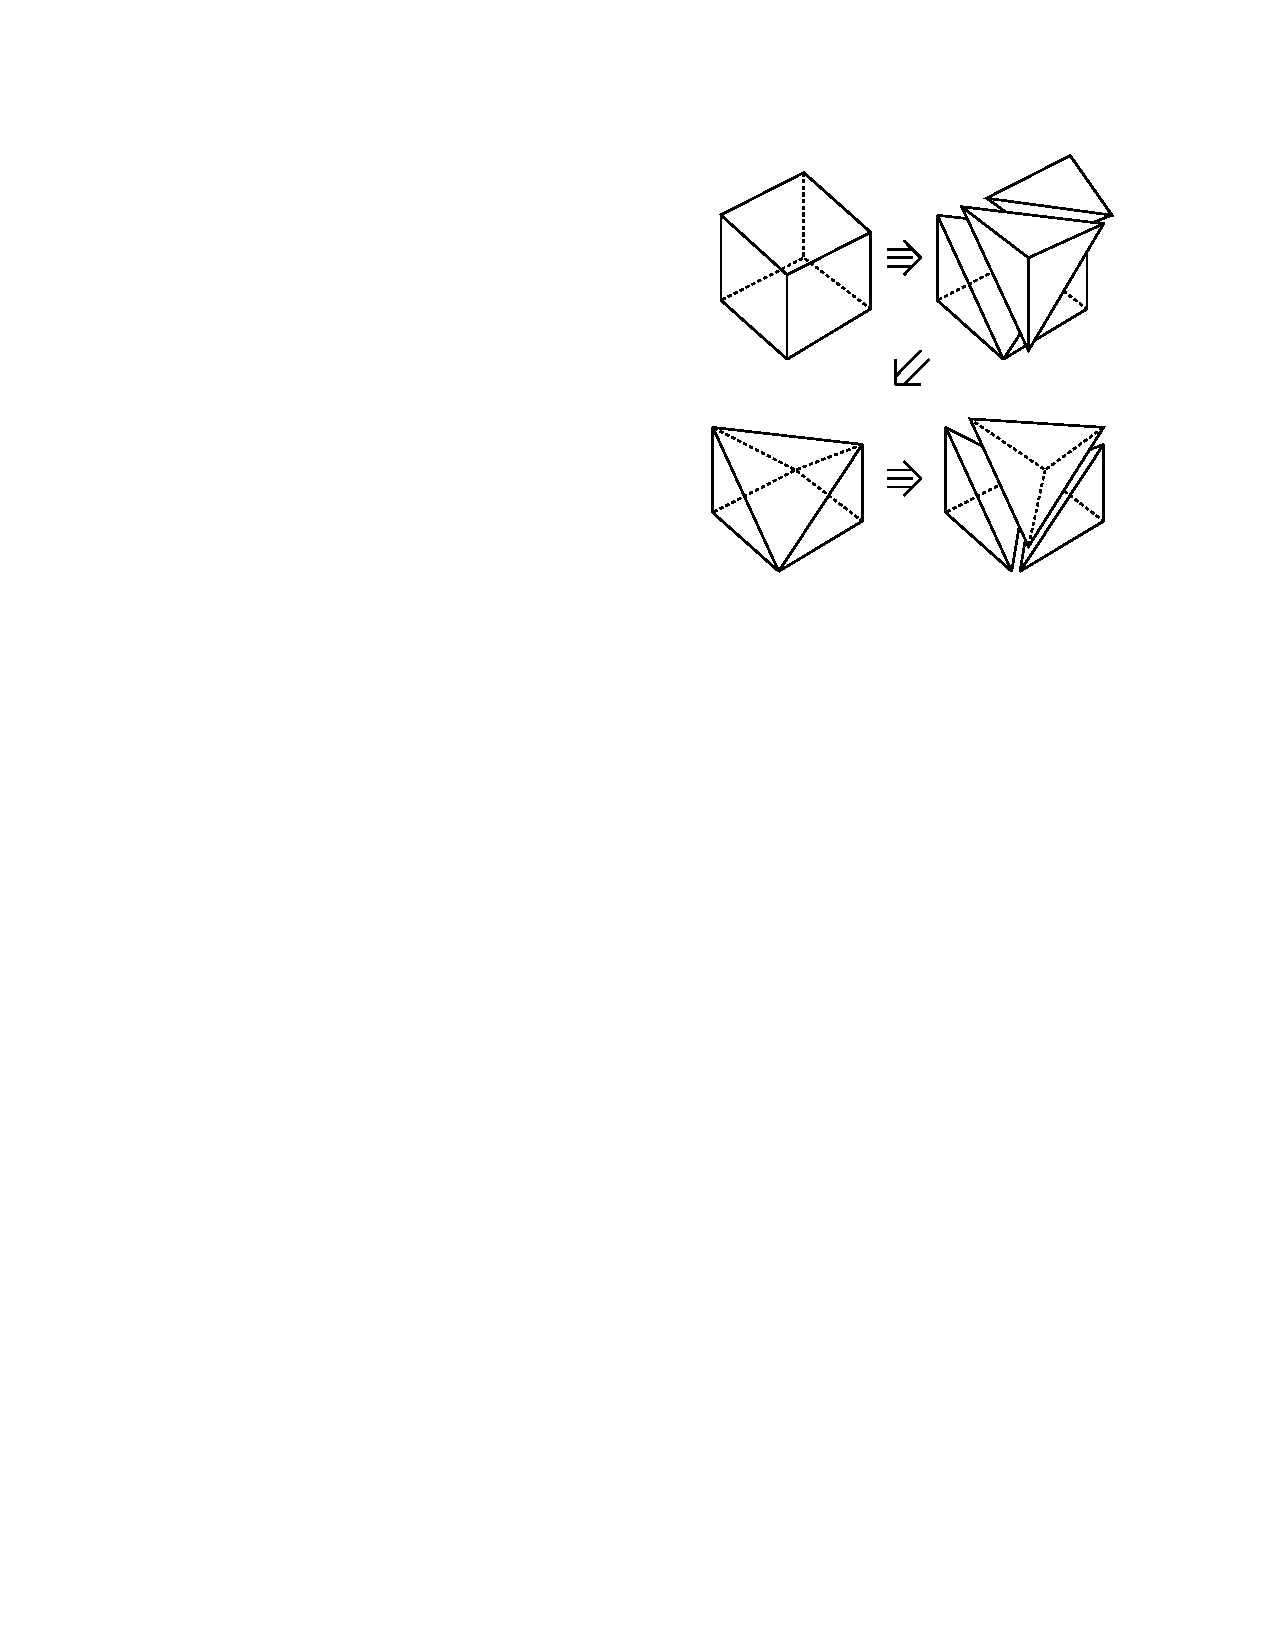
\includegraphics[width=0.6\textwidth]{img/04_cell_based_cropped}
        \caption{Decomposition of a cube into five tetrahedra. Source: A Polygonal Approximation to Direct Scalar Volume Rendering - [Shirley, Tuchmann 1990]}
\end{figure}


Cells are projected to \emph{triangle fans} consisting of
\begin{itemize}
    \item 1 \emph{thick vertex} (projection of the common edge of the tetrahedra)
    \item $3$ or $4$ \emph{thin vertices} (on the silhouette)
\end{itemize}
\begin{figure}[H]
    \centering
    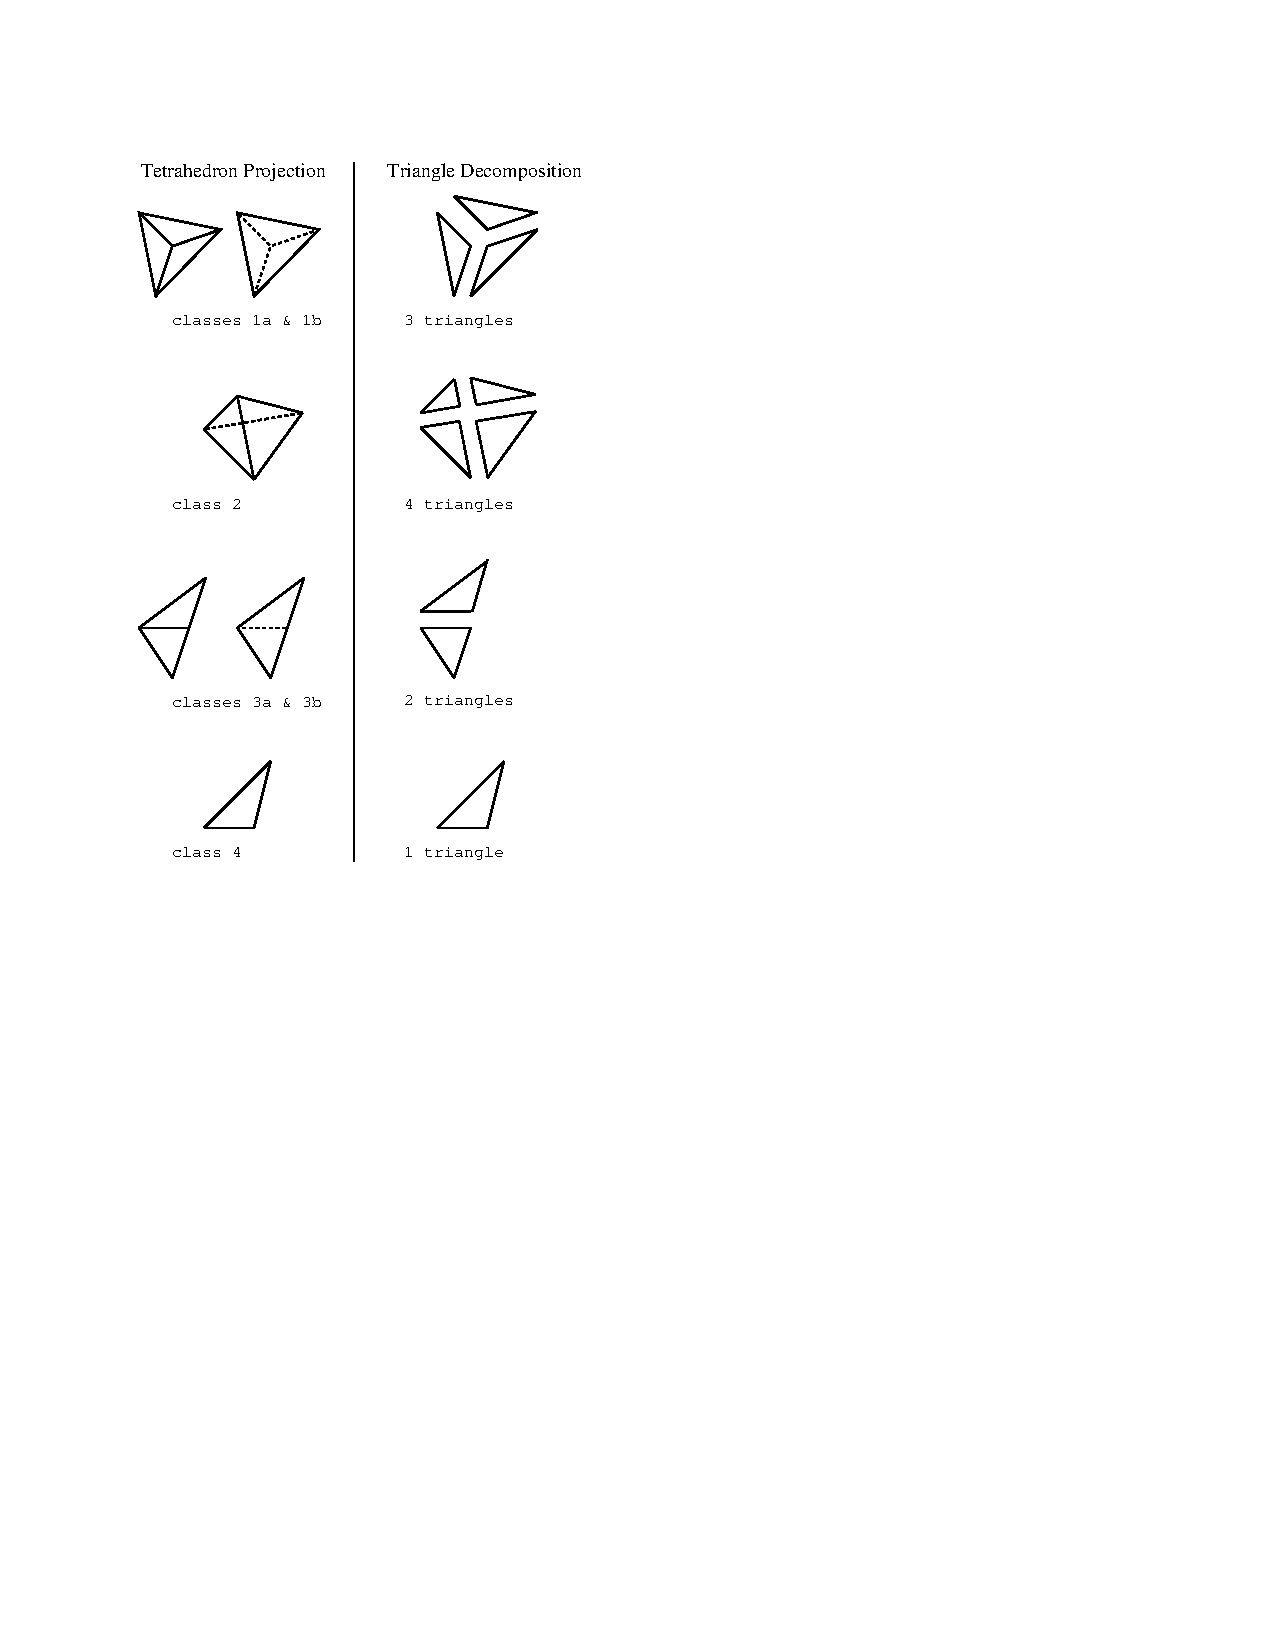
\includegraphics[width=0.6\textwidth]{img/04_cell_based_tetrahedra}
    \caption{Splitting tetrahedra. Source: A Polygonal Approximation to Direct Scalar Volume Rendering - [Shirley, Tuchmann 1990]}
\end{figure}

\paragraph{Original algorithm:} Store \emph{triangle fan} in \emph{space}:
\begin{itemize}
    \item Thin vertices are kept in the \emph{original position}.
    \item The thick vertex is set to the \emph{midpoint} of the projected edge.
\end{itemize}
Advantages:
\begin{itemize}
    \item \emph{Depth test} can be used (allows volume rendering into a scene).
    \item \emph{Viewing direction} and {field-of-view} can be changed (for a fixed camera position) by keeping the projection.
\end{itemize}

\paragraph{Computation of the thick vertex} $\ $
\begin{itemize}
    \item Compute the determinants 
        \begin{align*}
            d_i &= det(x_j, x_k, x_l) &i \in [0,3]
        \end{align*}
        where $x_j$, $x_k$ and $x_l$ are the vertices of the $i^{th}$ face relative to camera position, ordered counter clockwise on the outside of the face.
    \item If the number of positive determinants is 
        \begin{description}
            \item[Odd] Class 1
            \item[Even] Class 2
        \end{description}
    \item Interpolate weights 
\end{itemize}
\paragraph{Painting} The thick and thin vertices are then sent to the graphics card (with supplied texture coordinates). 
\subsubsection{Drawing}
\paragraph{Back-to-front compositing} $\ $
\begin{itemize}
    \item Cells must be depth-sorted $\Rightarrow$ visibility sorting.
    \item Drawing possible without re-sorting on camera turn and zoom.
    \item Depth-test (z-buffer) must be enabled.
    \item Additional (opaque) objects must be rendered before the volumes.
\end{itemize}
\paragraph{Visibility sorting} (MPVO algorithm, Williams 1992):
\begin{itemize}
    \item Generate \emph{partial ordering} of cells based on adjacent pairs.
    \item Break \emph{cycles} (rare, small rendering error, alternative: Split a cell).
    \item Sort the list of \emph{front cells} by distance to centroid (heuristic)
\end{itemize}

\subsubsection{Example: Visualisation of smoke propagation}
For this model we use a simple smoke model which is mostly used in fire protection engineering.
The \emph{absorption} $\tau$ is proportional to $s(x)$ (particle concentration). Which leads a to a simple preintegrated opacity transfer function:
\begin{align*}
    \alpha = 1-\exp\left( 
        - c {\tau_f+\tau_b \over 2}\norm{x_b - x_f}
    \right)
\end{align*}

\subsubsection{Opacities}
When compositing cells with low opacity then opacities are essentially \emph{added}. Adding many very small opacities (e.g. between $[0, 1/255]$) leads to \emph{quantisation artefacts}.
Options to reduce artefacts:
\begin{itemize}
    \item Compositing with $16$ bits
    \item \emph{$\alpha$-dithering} 
        use \emph{randomised rounding} instead of standard rounding:
        \begin{align*}
             x &\rightarrow \lfloor x \rfloor + \left( x - \lfloor x\rfloor \geq \text{rand} \right) &\text{with rand}\in [0,1]
        \end{align*}
        
\end{itemize}

\subsubsection{Hardware-Assisted Visibility Sorting}
HAVS, Silva et al. 2005 is a faster cell projection algorithm:
\begin{itemize}
    \item Requires $4$ RGBA float buffers for storing $7$ pairs of $(s,d)$ per pixel:
        \begin{itemize}
            \item With a scaler field value $s$,
            \item and distance $d$ to camera.
        \end{itemize}
    \item The initial cell sorting is done on the CPU based on the centroids. Which results in a
        \emph{$k$-nearly sorted sequence} with $k\leq 7$.
    \item Main loop: Draw all cell faces from back to front.
    \item Fragment shader:
        \begin{itemize}
            \item Insert $(s,d)$ into buffer
            \item If the buffer is full:
                \begin{itemize}
                    \item Take out furthes pair of $(s,d)$
                    \item Compute thickness of cell behind the pixel:
                        \begin{align*}
                            \Delta d = d-d_\text{old}
                        \end{align*}
                    \item Do a preintegrated TF lookup with $s$, $s_\text{old'}\Delta d$
                    \item Apply $\alpha$ compositing.
                \end{itemize}
        \end{itemize}
\end{itemize}















